% Appendix Template

\chapter{Résultats complémentaires} % Main appendix title

\label{Annexes1} % Change X to a consecutive letter; for referencing this appendix elsewhere, use \ref{AppendixX}

\lhead{Annexes 1. \emph{Résultats complémentaires}} % Change X to a consecutive letter; this is for the header on each page - perhaps a shortened title

\section{Tests de choix binaires}

\begin{figure}[ht]
\centering
		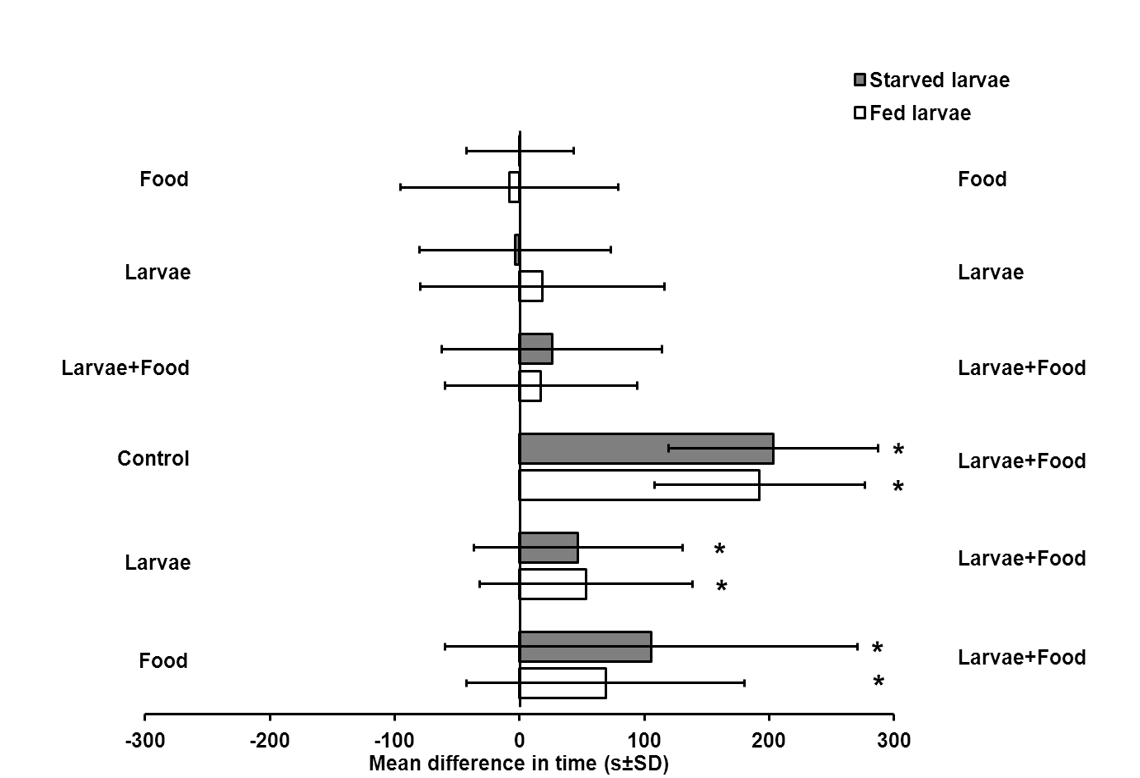
\includegraphics[width=1 \textwidth]{Figures/testchoixbinaire3.png}
		\rule{35em}{0.5pt}
		\caption[Exp2]{Combinaisons de choix binaires additionnelles à l'étude de \citet{boulay_evidence_2013} (cf. Chapitre \ref{Chapter2}). Différence du temps (moyenne $\pm$SD) passé les larves de \textit{Lucilia sericata} à jeûn (gris) et nourries (blanc) sur les signaux (moitié d'une zone) dans un test de choix binaire en individuel. La différence moyenne a été obtenue en soustrayant le temps passé sur le signal placé à droite de la figure à celui passé sur le signal placé à gauche. Si la différence est positive, les individus ont passé en moyenne plus de temps sur le signal placé à droite et inversement si la valeur est négative. Plus de détails sur le protocole sont à retrouver dans \citet{boulay_evidence_2013}. Les astérisques indiquent les différences significatives entre les zones (tests de Wilcoxon, N=20).}
	\label{fig:exp2}
    
\end{figure}


\begin{figure}[ht]
\centering
		
\includegraphics[width=0.8 \textwidth]{Figures/exp_pre1.png}
		\rule{35em}{0.5pt}
		\caption[Exp1]{Différence du temps (moyenne $\pm$SD) passé les larves de \textit{Lucilia sericata} (en noir) et \textit{Calliphora vomitoria} (en blanc) sur les signaux (moitié d'une zone) dans un test de choix binaire en individuel. La différence moyenne a été obtenue en soustrayant le temps passé sur le signal placé à droite de la figure à celui passé sur le signal placé à gauche. Si la différence est positive, les individus ont passé en moyenne plus de temps sur le signal placé à droite et inversement si la valeur est négative. Lu correspond à une zone marquée par 10 larves à jeun de \textit{L. sericata} pendant 10min, Ca correspond à une zone marquée par 10 larves de \textit{C. vomitoria}, et Control était une zone vierge de dépôt. Plus de détails sur le protocole sont à retrouver dans \citet{boulay_evidence_2013}. Les astérisques indiquent les différences significatives entre les zones (tests de Wilcoxon, N=20).}
	\label{fig:exp1}
    
\end{figure}


\clearpage


\section{Profil chromatographique du signal larvaire}

Un séjour d'une semaine a été fait au sein du Laboratoire de Chimie Analytique dans le Département Analyse Qualité et Risque dirigé par le Pr. G. \textsc{Lognay} (site de Gembloux Agro-Bio-Tech, Univ. de Liège) et en collaboration étroite avec F. \textsc{Verheggen} (Unité d'Entomologie fonctionnelle et évolutive, Gembloux Agro-Bio-Tech). Cette semaine a permis d'établir un protocole expérimental d'extraction du signal larvaire. Le solvant retenu a été une solution de chloroforme/méthanol reconcentré dans un mélange de dichlorométhane et d'héxane (50:50). Un premier profil chromatographique a été obtenu (Figure \ref{fig:chromato}) mettant en évidence une domination du cholestérol en terme d'abondance. 

\begin{figure}[ht]
\centering
		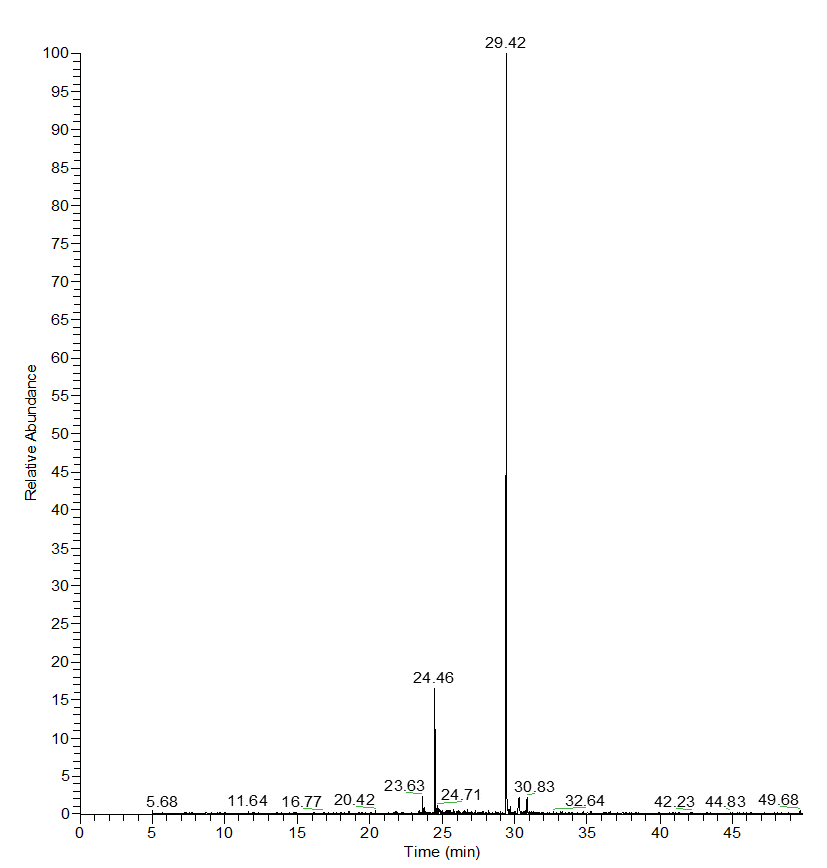
\includegraphics[width=0.8 \textwidth]{Figures/chromato.png}
		\rule{35em}{0.5pt}
		\caption[Chromato]{Profil chromatographique (GC-MS) du signal déposé par 20 larves de \textit{Lucilia sericata} durant 24h. Le composé majoritaire (pic à 29.42) a été identifié comme étant du cholestérol (Cholest-5-en-3-ol(3$\beta$)).}
	\label{fig:chromato}
    
\end{figure}

\section{Attraction à distance du groupe}
Des tests préliminaires en olfactomètre ont été réalisés avec un groupe de 40 larves de \textit{Lucilia sericata} versus un témoin (zone vide; cf. Figure \ref{fig:olfacto}). Les larves, testées individuellement, ont choisi dans 100$\%$ des cas la branche amenant au groupe. Le temps moyen de choix ($\pm$EcT) était de 258.2 $\pm$124s (N=10). Cette expérience préliminaire met en évidence l'existence d'un effet attractif à distance d'un groupe de larves sur les congénères. Cette attraction est vraisemblablement supportée par le signal larvaire. Des tests supplémentaires seront à réaliser pour affirmer ou infirmer cette hypothèse.

\begin{figure}[ht]
\centering
		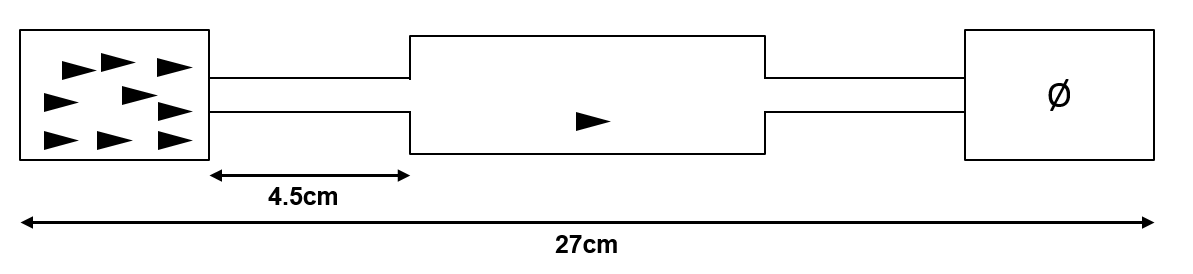
\includegraphics[width=0.8 \textwidth]{Figures/olfacto.png}
		\rule{35em}{0.5pt}
		\caption[Olfacto]{Dispositif d'olfactométrie utilisé pour tester l'effet attractif à distance d'un groupe de 40 larves de \textit{Lucilia sericata} sur des congénères.}
	\label{fig:olfacto}
    
\end{figure}
 
 
 
 
 
